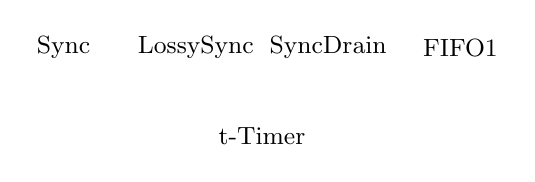
\begin{tikzpicture}[scale=1.4]

\tikzstyle{every node}=[font=\small]
\tikzstyle{label}=[draw=none]

\draw (0.5, -0.3) node[label] {Sync};
\draw (1.7, -0.3) node[label] {LossySync};
\draw (2.9, -0.3) node[label] {SyncDrain};
\draw (4.1, -0.3) node[label] {FIFO1};
\draw (2.3, -1.1) node[label] {t-Timer};

\sync{(0,0)}{(1,0)}{}
\lossysync{(1.2,0)}{(2.2,0)}{}
\syncdrain{(2.4,0)}{(3.4,0)}{}
\fifoe{(3.6,0)}{(4.6,0)}{}

\timer{(1.8,-0.8)}{(2.8,-0.8)}{node [above left] {t}}

\end{tikzpicture}
